\chapter{模擬實驗與結果分析}\label{Experimental_results}


\section{感測器數量}

圖\ref{fig_tikzpicture_demo}為透過 $LaTeX$ 套件 tikzpicture 繪製出的圖形。圖\ref{fig_nkust} 為 JPEG 格式之圖片。圖\ref{fig_taiwan_symbol} 為去背的 PNG 格式圖案,圖\ref{fig_nkust}\cite{nkust_jpg}與圖\ref{fig_taiwan_symbol}\cite{taiwan_symbol}資料來源為中文維基百科。


\begin{figure}[htbp]
    \centering
    \begin{tikzpicture}
        \begin{axis}[
            tick scale binop=\times,
            % title={Number of Nodes},
            xlabel={$Number of Nodes$},
            ylabel={$Total Weight$},
            legend entries={$a$, $b$},
            xmin=100, ymin=0,
            xmax=500,
            %ymax=120,
            xtick={100,200,300,400,500},
            %ytick={0,20,40,60,80,100,120},
            legend pos=outer north east, %outer north east, north west, north east, south west, south east
            ymajorgrids=true,
            grid style=dashed, %solid, (densely, loosely) dotted, (densely, loosely) dashed, (densely, loosely) dashdotted, (densely, loosely) dashdotdotted, {color=blue, thick}
            legend style={cells={anchor=west}},%align text left
            % legend style={font=\large},
            % legend style={draw=none}, without legend box
            % legend style={legend columns=-1}, draw legend horizontally    
            % legend style={at={(1,0.5)}, anchor=east},
            % line width=1.0pt,
            % mark size=2.0pt,
        ]

        % none
        % +, *, o, x, triangle, cube(square), star, diamond, otimes, oplus, pentagon, |, halfcircle, ball
        % triangle*, cube*, diamond*, square*, halfcircle*, halfsquare* (halfdiamond*), pentagon*, halfsquare right*, halfsquare left*

        % red, green, blue, cyan, magenta, yellow, black,
        % gray, white, darkgray, lightgray, brown, lime,
        % olive, orange, pink, purple, teal, violet.
        % red!30!white implies that 30% of red and 70% of white
        % rgb,255:red,231;green,84;blue,121 implies that 231/255 red, 84/255 green, and 121/255

        %solid, (densely, loosely) dotted, (densely, loosely) dashed, (densely, loosely) dashdotted, (densely, loosely) dashdotdotted

        \addplot[
            color=gray,
            densely dashed,
            mark=+,
            mark options={solid},
        ] table from {./Figures/Result/alpha001.txt};

        \addplot[
            color=red,
            densely dotted,
            mark=triangle*,
            mark options={solid},
        ] table from {./Figures/Result/alpha010.txt};

        % \addplot[
        %     color=blue!50,
        %     solid,
        %     mark=o,
        %     mark options={solid},
        % ] table {alpha100.txt};
        \end{axis}
    \end{tikzpicture}
    \caption{tikzpicture Demo}
    \label{fig_tikzpicture_demo}
\end{figure}


\begin{figure}[H] 
    \centering 
    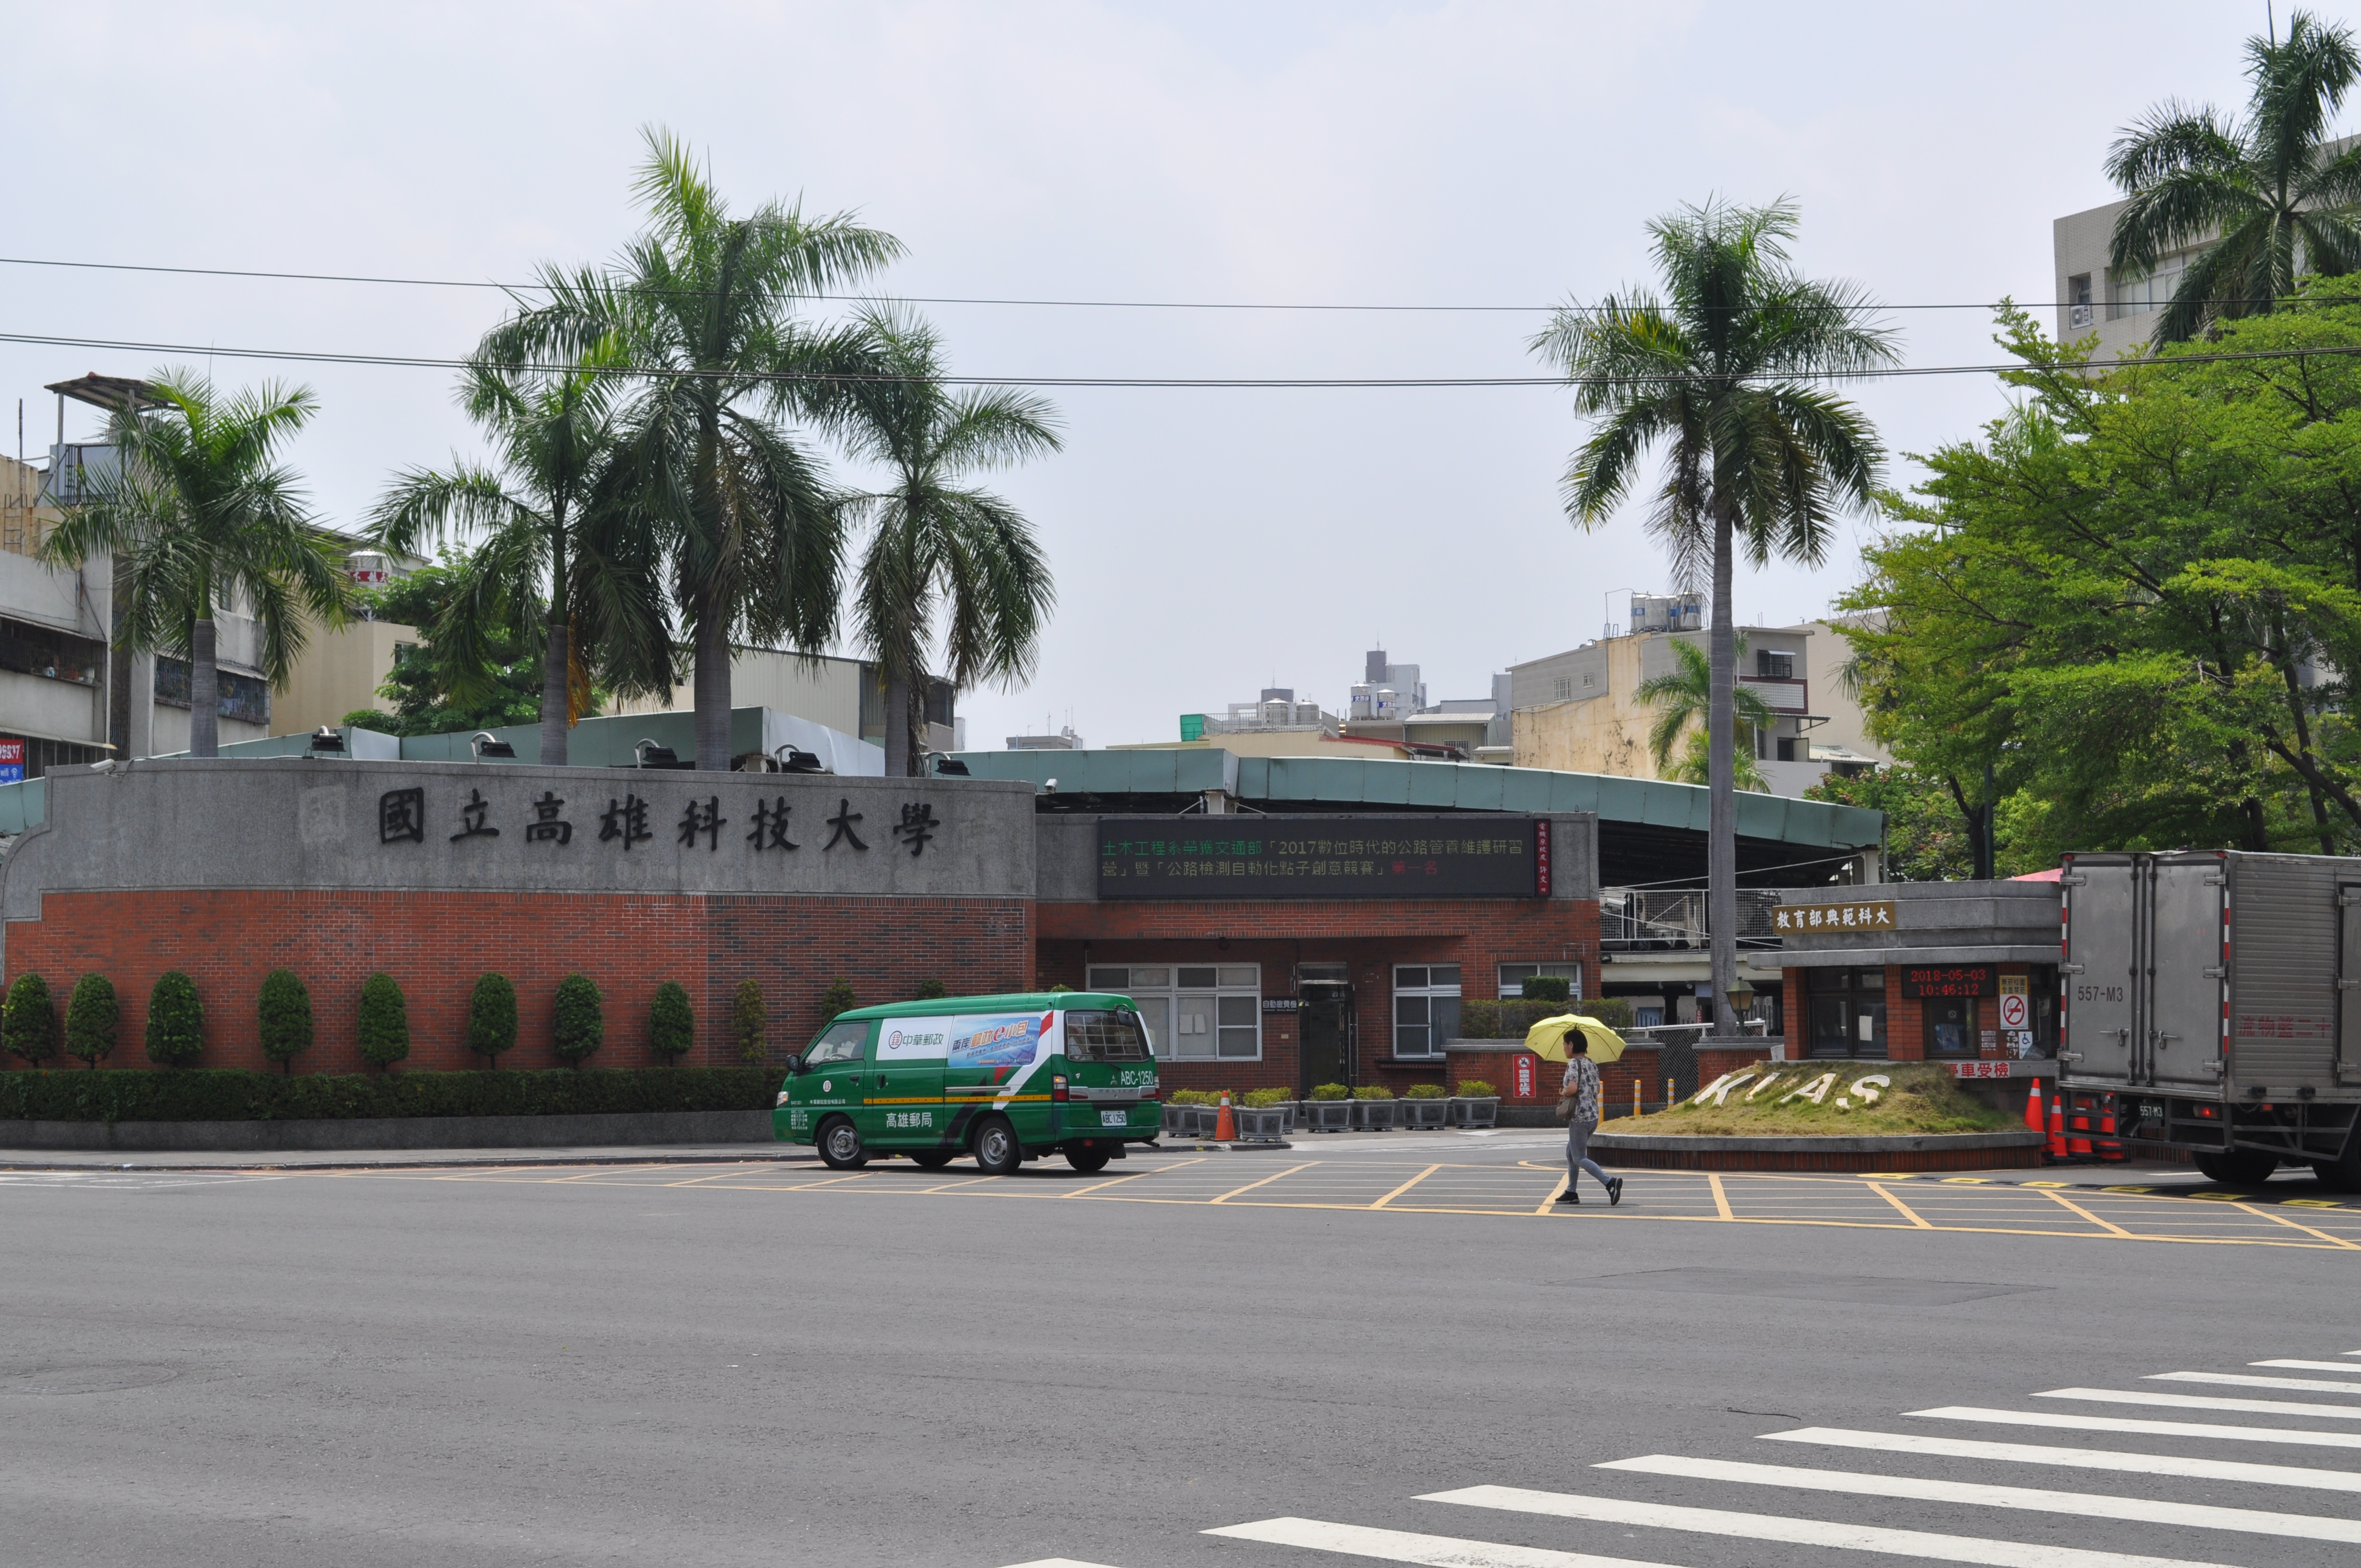
\includegraphics[width=0.5\textwidth]{./Figures/ImageTest/NKUST.jpg} 
    \caption{NKUST 校門口}
    \label{fig_nkust}
\end{figure}

\begin{figure}[H] 
    \centering 
    \includegraphics[width=0.7\textwidth]{./Figures/ImageTest/Taiwan_symbol.png} 
    \caption{Taiwan symbol}
    \label{fig_taiwan_symbol}
\end{figure}

圖\ref{fig_nkust_logo}為國立高雄科技大學校徽集,圖\ref{fig_nkust_logo_1}與圖\ref{fig_nkust_logo_4}為外加方格的校徽,圖\ref{fig_nkust_logo_2}與圖\ref{fig_nkust_logo_3}為無外加方框的校徽,圖片來源來自於 NKUST 形象識別系統(校徽)\cite{logo}。

\begin{figure}[H]
    \centering 
    \subfigure[校徽]{
        \setlength{\fboxrule}{0.5pt}
        \fbox{\includegraphics[width=5.5cm]{./Figures/ImageTest/f4.png}}
        \label{fig_nkust_logo_1}
    }
    \quad
    \subfigure[校徽特別範例]{
        \setlength{\fboxrule}{0.5pt}
        \includegraphics[width=5.5cm]{./Figures/ImageTest/f5.png}
        \label{fig_nkust_logo_2}
    }
    \quad
    \subfigure[英文簡稱/上下組合]{
        \setlength{\fboxrule}{0.5pt}
        \includegraphics[width=5.5cm]{./Figures/ImageTest/f6.png}
        \label{fig_nkust_logo_3}
    }
    \quad
    \subfigure[中文全銜、英文簡稱/上下組合]{
        \setlength{\fboxrule}{0.5pt}
        \fbox{\includegraphics[width=5.5cm]{./Figures/ImageTest/f7.png}}
        \label{fig_nkust_logo_4}
    }
    \caption{NKUST Logo}
    \label{fig_nkust_logo}
\end{figure}


\section{表格測試}
\begin{table} [!h]
    \centering
    \centering \caption{Summary of Notations}
    \begin{tabular}{|p{1.5cm}|p{6.5cm}|} \hline
    Symbol &Definition
    \\ \hline
    $n$& the number of nodes in $G$
    \\ \hline
    $v.hop$& the minimum
    \\ \hline
    \end{tabular}\label{table:notation}
    
\end{table}

% \newpage